\documentclass[12pt,a4paper]{article}
\usepackage[utf8]{inputenc} 
\usepackage[T1]{fontenc}		       
\usepackage{lmodern}			       
\usepackage{babel} 
\usepackage{amsmath}
\usepackage{amsfonts}
\usepackage{amssymb}
\usepackage{graphicx}
\usepackage{xcolor}
\usepackage{mathtools}
\usepackage{fancyhdr}
\usepackage{enumitem}
\usepackage{tcolorbox}
\usepackage{stmaryrd}
\usepackage{dsfont}
\usepackage{pgf, tikz}
\usepackage[linesnumbered,ruled,vlined]{algorithm2e}
\usepackage[text={15cm,24.5cm},centering]{geometry}

% Définir le texte affiché en fin de page
\pagestyle{fancy}
\fancyhf{}  % Clear the default headers and footers
\rfoot{\hrule
    \vspace{0.3cm}
    \noindent\textsf{Félix de Brandois}
    \hfill \thepage
}
\renewcommand{\headrulewidth}{0pt}

% Style de l'entete
\newcommand{\entete}{
    \noindent\textbf{INSA - ModIA, 4$^e$ année.}
    \hfill \textbf{Années 2023-2024}
    
    \begin{center}
        \textbf{\LARGE Machine Learning}
    \end{center}
}


% Définir la fonction pour créer une boîte de propriété
\newcommand{\propriete}[2]{%
    \begin{tcolorbox}[colback=white,colframe=green!25!white,title=\textbf{Propriété #1}, coltitle=black]
        #2
    \end{tcolorbox}
}

% Définir la fonction pour créer une boîte de définition
\newcommand{\definition}[2]{%
    \begin{tcolorbox}[colback=white,colframe=blue!25!white,title=\textbf{Définition #1}, coltitle=black]
        #2
    \end{tcolorbox}
}

% Définir la fonction pour créer une boîte de théorème
\newcommand{\theoreme}[2]{%
    \begin{tcolorbox}[colback=white,colframe=red!25!white,title=\textbf{Théorème #1}, coltitle=black]
        #2
    \end{tcolorbox}
}

% Définir la fonction pour créer une boîte de remarque
\definecolor{customRed}{RGB}{150, 30, 30}
\newcommand{\remarque}[1]{%
    \leftline{\noindent
    \textcolor{customRed}{\vrule width 3pt}\hspace{10pt}%
    \parbox{0.9\textwidth}{%
        \textbf{Remarque :}
        #1
    }}
    \vspace{10pt}
}

% Définir la fonction pour créer une boîte de preuve
\newcommand{\preuve}[1]{%
    \begin{quote}
        $\blacktriangleright$~#1
    \end{quote}
}

% Définir la fonction pour créer un encadrement de texte
\newcommand{\important}[1]{%
    \begin{tcolorbox}[colback=red!10!white,colframe=red!30!black]
        #1
    \end{tcolorbox}
}



\begin{document}

\entete

\vspace{0.5cm}

\section{Introduction}

\subsection{Binary Classification problem}

\important{
    \vspace{-\baselineskip}\begin{align*}
        \text{Find a binary classifier : } \quad h : \mathbb{R}^n &\to \{-1, 1\} \hspace{14.5cm} \\
        x &\mapsto h(x)\vspace{-\baselineskip}
    \end{align*}
    So that $\mathbb{P}_{(x, y) \sim D} [h(x) \neq y]$ is small.\\
    With :
    \begin{itemize}
        \item $X$ : space of input data (image, text, sound, etc.)
        \item $Y$ : space of label (e.g. $Y = \{-1, 1\}$)
        \item $D$ : joint probability distribution of $(x, y) \in X \times Y$
    \end{itemize}
}

\fbox{\textbf{$\rightarrow$ Objectif of ML : } Risk Minimization for $h \in H$}\\

\definition{- Test error of $h$}{
    Let $h \in H$, the test error of $h$ is defined as :
    \begin{align*}
        R_D(h) &= \mathbb{E}_{(x, y) \sim D} [\mathds{1}_{h(x) \neq y}] \\
        &= \int_{X \times Y} \mathds{1}_{h(x) \neq y} \, D(dx, y)
    \end{align*}
}

\propriete{- Bayes Classifier}{
    The minimal risk is given by the Bayes Classifier :
    $$
        h_{\text{Bayes}} = \underset{y \in \{-1, 1\}}{\text{argmax }} \mathbb{P}_{(x, y) \sim D} [y|x] \in \{-1, 1\}
    $$
}

\noindent\textbf{Example :} 
$\mathbb{P}(y | x)$ with gaussians mixitures \\

Let $\mathbb{P}(y = -1) = \pi_0, \qquad 
\mathbb{P}(y = 1) = 1 - \pi_0 \qquad \text{with } \pi_0 \in [0, 1]$\\
$\mathbb{P}(x|y = -1) = \mathcal{N}(\mu_1, \Sigma_1), \qquad 
\mathbb{P}(x|y = 1) = \mathcal{N}(\mu_2, \Sigma_2)$\\

\begin{align*}
    \mathbb{P}(y = -1 | x) &= \frac{\mathbb{P}(x | y = -1)\mathbb{P}(y = -1)}{\mathbb{P}(x)} \qquad \text{(Bayes' rule)} \\
    &= \frac{\mathbb{P}(x | y = -1)\mathbb{P}(y = -1)}{\mathbb{P}(x | y = -1)\mathbb{P}(y = -1) + \mathbb{P}(x | y = 1)\mathbb{P}(y = 1)} \\
    & \\
    \mathbb{P}(y = 1 | x) &= 1 - \mathbb{P}(y = -1 | x)
\end{align*}

Therefore,
\begin{align*}
    & h_{\text{Bayes}} (x) = \begin{cases}
        1 & \text{if } \mathbb{P}(y = 1 | x) > \mathbb{P}(y = -1 | x) \\
        -1 & \text{if } \mathbb{P}(y = 1 | x) < \mathbb{P}(y = -1 | x) \\
        \pm 1 & \text{if } \mathbb{P}(y = 1 | x) = \mathbb{P}(y = -1 | x)
    \end{cases}\\
    \Leftrightarrow \quad & h_{\text{Bayes}} (x) = \text{sign}(\mathbb{P}(x | y = -1) \pi_0 - \mathbb{P}(x | y = 1)(1 - \pi_0))
\end{align*}



\theoreme{}{
    Let $H$ be all measurable functions from $X$ to $\{-1, 1\}$. \\
    Then, $R_D(h) \geq R_D(h_{\text{Bayes}})$ for all $h \in H$.
}

\preuve{
    Assume $D(dx, y) = \mathbb{P}(x | y)dx \cdot \mathbb{P}(y) = \mathbb{P}(y | x)\mathbb{P}(x)dx$
    \begin{align*}
        \text{Then : } \quad R_D(h) &= \mathbb{E}_{(x, y) \sim D} [\mathds{1}_{h(x) \neq y}] \\
        &= \sum_{y \in \{-1, 1\}} \int_X \mathds{1}_{h(x) \neq y} D(dx, y) \\
        &= \sum_{y \in \{-1, 1\}} \int_X \mathds{1}_{h(x) \neq y} \mathbb{P}(y | x)\mathbb{P}(x)dx \\
        &= \int_X \mathbb{P}(y = 1 | x) \mathds{1}_{h(x) \neq 1} \mathbb{P}(x)dx + \int_X \mathbb{P}(y = -1 | x) \mathds{1}_{h(x) \neq -1} \mathbb{P}(x)dx \\
    \end{align*}
}

\textit{Texte manquant}



\subsection{Linear Classification problem}

In general, $D$ is unknown and $\mathbb{P}(x|y)$ is hard to model, $\mathbb{P}(y)$ prior to choose.\\
Start from "simple" $H$ : linear classifiers on $x \in \mathbb{R}^n$.

\definition{- Linear classifier}{
    A linear classifier is a function $h : \mathbb{R}^n \to \{-1, 1\}$ of the form :
    \begin{align*}
        h(x) &= \text{sign}(\langle w, x \rangle + b) \\
        &= \text{sign}(\sum_{i = 1}^n w_i x_i + b)
    \end{align*}
    with $w \in \mathbb{R}^n$ and $b \in \mathbb{R}$.
}

\remarque{ Labels : \\
    $+1$ if $w^Tx + b > 0$\\
    $-1$ if $w^Tx + b < 0$\\
    $\pm 1$ if $w^Tx + b = 0$
}

\vspace{0.5cm}

\begin{tcolorbox}[colback=red!10!white,colframe=red!30!black]
    Given a set of training samples iid from $D$ : \\
    $S = \{(x_1, y_1), \dots, (x_m, y_m)\} \in (X \times Y)^m$\\
    Find a classifier $h_S \in H$ such that the generalization error $R_D(h_S)$ is small.
\end{tcolorbox}

\begin{algorithm}
    \caption{Perceptron}
    \vspace{0.2cm}
    Initialize $k = 0$ and $w_0 \in \mathbb{R}^n$\\
    \Repeat{}{
        \For{$i = 1, \dots, m$}{
            \If{sign($w_k^T x_i) = y_i$}{
                exit if $k$ big
            }
            \Else{
                \If{$y_i = 1$}{
                    $w_{k + 1} = w_k + x_i$\\
                }
                \Else{
                    $w_{k + 1} = w_k - x_i$\\
                }
            }
        }
        $k = k + 1$
    }
\end{algorithm}

\remarque{
    $k$ is the number of iterations or the number of errors made by the algorithm.
}

\remarque{
    $S$ can be separated by some $h \in H$.\\
    i.e. $\exists w^* \in \mathbb{R}^n$ so that $||w^*|| = 1$ and $\forall i \in \{1, \dots, m\}, y_i(w^{*T}x_i) > 0$.
}

\theoreme{}{
    On linear separable data $S$ and $w_0 = 0$, the Perceptron algorithm generates $(w_k)_{k \geq 0}$ which converges in finite number of error corrections.
}

\preuve{
    Let $\forall i \leq m, y_i = \text{sign}(\langle w^*, x_i \rangle)$\\
    Let $R = \underset{i \leq m}{\text{max }} ||x_i|| < \infty$ and $M = \underset{i \leq m}{\text{min }} y_i \langle w^*, x_i \rangle > 0$\\

    We have to show that $\langle w_{k + 1}, w^* \rangle \geq \langle w_k, w^* \rangle + M$\\
    Indeed, if $y_i = 1$ and $\text{sign}(\langle w_k, x_i \rangle) = -1$ then :
    \begin{align*}
        &w_{k + 1} = w_k + x_i \text{ and } \langle w^*, x_i \rangle \geq M \\
        \Rightarrow &\langle w_{k + 1}, w^* \rangle = \langle w_k, w^* \rangle + \langle x_i, w^* \rangle \geq \langle w_k, w^* \rangle + M
    \end{align*}
    Similarly, if $y_i = -1$.

    Therefore, $\langle w_k, w^* \rangle \geq kM$ and $||w_k|| \sim \mathcal{O}(\sqrt{k})$.

    Then, $\frac{\langle w_k, w^* \rangle}{||w_k||} \geq \frac{kM}{\sqrt{k}R} \geq \frac{M}{R} \sqrt{k}$ and $\langle w_k, w^* \rangle \leq ||w_k|| \cdot ||w^*|| \leq ||w_k||$.\\
    So, $k \leq \left(\frac{R}{M}\right)^2$.
}

\remarque{
    $M$ is the margin of the data.\\
    $M = \underset{i \leq m}{\text{min }} y_i \langle w^*, x_i \rangle$
    $\qquad M \nearrow \Rightarrow k_{\text{max}} \searrow$\\
}

\remarque{
    Unclear if the the Perceptron algorithm finds $h_{\text{Bayes}}$ which minimize the test error.\\
    Unclear if $S$ non linear separable $(M \leq 0)$.\\

    Extend algo to $H = \{\bar{x} \mapsto \text{sign}(\bar{w}^T \bar{x}) + \bar{b} | \bar{w} \in \mathbb{R}^n, \bar{b} \in \mathbb{R}\}$.\\
    Consider $\bar{x} = (x, 1) \in \mathbb{R}^{n + 1}$ and $\bar{w} = (w, b) \in \mathbb{R}^{n + 1}$.
}

\section{Support Vector Machine}

\important{
    Find a linear classification which has a maximal margin.\\
    $\Rightarrow$ Smallest test error.
}

\definition{- Margin}{
    Let $w \in \mathbb{R}^n$ and $b \in \mathbb{R}$, the margin of $(w, b)$ is :
    $$
        \phi_h = \underset{i \leq m}{\text{min }} \frac{||w^T x_i + b||}{||w||}
    $$
}

\subsection{Problem formulation}

\subsubsection{Linearly separable case}

$$
\underset{w \in \mathbb{R}^n, b \in \mathbb{R}}{\text{max }} \phi_h \quad \text{ so that } \quad \forall i \leq m, y_i(w^T x_i + b) > 0
$$
Feasible solution exists : $\exists w \in \mathbb{R}^n, b \in \mathbb{R}$ so that $\forall i \leq m, y_i(w^{T}x_i + b) > 0$.\\

\important{
    Reformulation of SVM :\\
    $$
    \underset{w \in \mathbb{R}^n, b \in \mathbb{R}}{\text{max }} \underset{i \leq m}{\text{min }} \frac{y_i(w^T x_i + b)}{||w||}
    $$
}

\remarque{
    Invariance by scaling : $\forall \lambda > 0, (w, b)$ solution $\Rightarrow (\lambda w, \lambda b)$ solution. \\
    $\Rightarrow$ Set $\underset{i \leq m}{\text{min }} y_i(w^T x_i + b) = 1$.
}

\important{
    Formulation of SVM :
    \begin{equation}
        (P) \qquad \underset{w \in \mathbb{R}^n, b \in \mathbb{R}}{\text{max }} \frac{1}{||w||} \quad \text{ so that } \quad \underset{i \leq m}{\text{min }} y_i(w^T x_i + b) = 1
    \end{equation}

    \begin{equation}
        (P') \qquad \underset{w \in \mathbb{R}^n, b \in \mathbb{R}}{\text{max }} \frac{1}{||w||} \quad \text{ so that } \quad \forall i \leq m, y_i(w^T x_i + b) \geq 1
    \end{equation}
}

\propriete{}{
    $(P)$ and $(P')$ are equivalent.
}

\preuve{
    \vspace{-\baselineskip}
    \begin{itemize}
        \item If $(\bar{w}, \bar{b})$ is a solution of $(P')$, then it is a feasible solution of $(P)$.\\
        \begin{itemize}
            \item If $\underset{i \leq m}{\text{min }} y_i(\bar{w}^T x_i + \bar{b}) = 1$, then $(P') \Rightarrow (P)$.
            \item If $\underset{i \leq m}{\text{min }} y_i(\bar{w}^T x_i + \bar{b}) > 1$ : \\
            Let $\phi_{\bar{w}, \bar{b}} = \underset{i \leq m}{\text{min }} \frac{y_i(\bar{w}^T x_i + \bar{b})}{||\bar{w}||} > \frac{1}{||\bar{w}||}$.\\
            Let $\hat{w} = \frac{\bar{w}}{||\bar{w}||} \frac{1}{\phi_{\bar{w}, \bar{b}}}$ and $\hat{b} = \frac{\bar{b}}{||\bar{w}||} \frac{1}{\phi_{\bar{w}, \bar{b}}}$\\
            Then, $\underset{i \leq m}{\text{min }} y_i(\hat{w}^T x_i + \hat{b}) = 1$ and $\frac{1}{||\hat{w}||} < \frac{1}{||\bar{w}||}$. So $(\bar{w}, \bar{b})$ is not optimal for $(P')$ : absurd.
        \end{itemize}

        \item $\forall (w, b)$ so that $\underset{i \leq m}{\text{min }} y_i(w^T x_i + b) = 1$ (solution of $(P)$), we have :\\
        $\frac{1}{||\bar{w}||} \geq \frac{1}{||w||}$ (by optimality of (P')).\\
        So $(\bar{w}, \bar{b})$ is a solution of $(P')$.
    \end{itemize}
}

\important{
    Primal problem :
    \begin{equation}
        (P'') \qquad \underset{w \in \mathbb{R}^n, b \in \mathbb{R}}{\text{min }} \frac{1}{2} ||w||^2 \quad \text{ so that } \quad \forall i \leq m, y_i(w^T x_i + b) \geq 1
    \end{equation}
}

\remarque{
    $(P'') \Leftrightarrow (P')$\\
    $(P'')$ is a quadratic programming with linear constraints.
}

\remarque{
    We can deduce the dual problem of $(P'')$ with KKT.
}

\subsubsection{Extension to non-linearly separable data}

\important{
    \begin{equation}
        \underset{w \in \mathbb{R}^n, b \in \mathbb{R}, \xi \in \mathbb{R}^m}{\text{min }} \frac{1}{2} ||w||^2 + C \sum_{i = 1}^m \xi_i^p \quad \text{ so that } \quad \forall i \leq m, y_i(w^T x_i + b) \geq 1 - \xi_i
    \end{equation}
    With :
    \begin{itemize}
        \item $C > 0$ : regularization parameter
        \item $\xi_i \geq 0$ : slack variable
        \item $p \geq 1$ : norm of the slack variable
    \end{itemize}
}

\section{Generalisation theory in binary classification}

\important{
    Find $h \in H$ so that $R_D(h) = \mathbb{P}_{(x, y) \sim D} [h(x) \neq y]$ is small.\\
} 

Given a set of training samples iid from $D$ : $S = \{(x_1, y_1), \dots, (x_m, y_m)\} \in (X \times Y)^m$\\
$h_s \in H$ is the classifier learned from an algorithm (Perceptron, SVM, etc.)\\

\propriete{}{
    \begin{equation}
        \underset{h \in H}{\text{min }} \frac{1}{m} \sum_{i = 1}^m \mathds{1}_{h(x_i) \neq y_i} \xrightarrow[m \to \infty]{\text{Loi des Grands Nombres}} R_D(h)
    \end{equation}
}

Classical picture of ML theory :\\

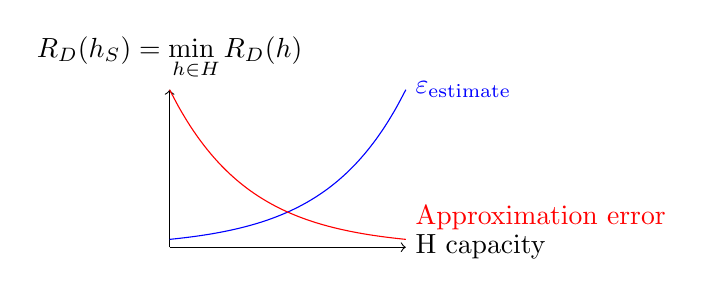
\begin{tikzpicture}
    \draw[->] (0, 0) -- (3, 0) node[right] {H capacity};
    \draw[->] (0, 0) -- (0, 2) node[above] {$R_D(h_S) = \underset{h \in H}{\text{min }} R_D(h)$};
    \draw[domain=0:3, smooth, variable=\x, blue] plot ({\x}, {2*exp(\x - 3)}) node[right] {$\varepsilon_{\text{estimate}}$};
    \draw[domain=0:3, smooth, variable=\x, red] plot ({\x}, {2*exp(-\x)}) node[above right] {Approximation error};
\end{tikzpicture}

Overfitting :\\
$R_D(h_S)$ big but $\frac{1}{m} \sum_{i = 1}^m \mathds{1}_{h(x_i) \neq y_i} \approx 0$\\


\textit{Texte manquant}


\underline{How to analyse $R_D(h_S)$ ?}

$S$ iid from $D \Rightarrow h_S$ is a random variable $\Rightarrow R_D(h_S)$ is a random variable.

\begin{enumerate}
    \item Control of $\mathbb{E}_{S \sim D^m} [R_D(h_S)]$
    \item Confidence interval for $R_D(h_S)$\\
\end{enumerate}

\subsection{Control of $\mathbb{E}_{S \sim D^m} [R_D(h_S)]$}

Leave-one-out cross-validation analysis for linear separable data :\\
$\mathbb{P}_{S \sim D^m} [S \text{ linear separable}] = 1$.

Leave-one-out algo A : $h_S = A(S)$\\

$\hat{R}_{\text{LOO}}(A) = \frac{1}{m} \sum_{i = 1}^m \mathds{1}_{h_{S \backslash \{x_i\}}(x_i) \neq y_i}$\\

\propriete{}{
    If $m \geq 2$, then $\mathbb{E}_{S \sim D^m} [\hat{R}_{\text{LOO}}(A)] = \mathbb{E}_{S' \sim D^{m - 1}} [R_D(h_S')]$
}

\preuve{
    \vspace{-\baselineskip}
    \vspace{-\baselineskip}
    \begin{align*}
        \mathbb{E}_{S \sim D^m} [\hat{R}_{\text{LOO}}(A)] &= \mathbb{E}_{S \sim D^m} \left[\frac{1}{m} \sum_{i = 1}^m \mathds{1}_{h_{S \backslash \{x_i\}}(x_i) \neq y_i}\right] \\
        &= \frac{1}{m} \sum_{i = 1}^m \mathbb{E}_{S \sim D^m} [\mathds{1}_{h_{S \backslash \{x_i\}}(x_i) \neq y_i}] \\
        &= \mathbb{E}_{S \sim D^m} [\mathds{1}_{h_{S \backslash \{x_1\}}(x_1) \neq y_1}] \qquad \text{(by independence)} \\
        &= \mathbb{E}_{S' \sim D^{m - 1}} [\mathbb{E}_{(x, y) \sim D} [\mathds{1}_{h_{S'}(x) \neq y}]] \qquad (S' = S \backslash \{x_1\}) \\
        &= \mathbb{E}_{S' \sim D^{m - 1}} [R_D(h_{S'})]
    \end{align*}
}

\theoreme{}{
    Assume $S$ is linearly separable (almost surely).\\
    Let $N_{\text{sn}}(S) = |\{x_i | y_i(w^T x_i + b) = 1, i \leq m\}|$ (number of support vectors).\\
    Then, $\mathbb{E}_{S \sim D^m} [\hat{R}_{\text{LOO}}(A)] \leq \mathbb{E}_{S \sim D^m} [\frac{N_{\text{sn}}(S)}{m}]$
}

\preuve{
    Let $(x, y) \in S$. If $x$ is not a support vector of $h_S$ : $h_{S \backslash \{x\}} = h_S$.\\
    Therefore, if $h_{S \backslash \{x\}}(x) \neq y$ then $x$ is a support vector of $h_S$.\\
    So, $\hat{R}_{\text{LOO}}(h_S) \leq \frac{N_{\text{sn}}(S)}{m}$.
}



\end{document}